\section{Keep-alive Tradeoffs}
\label{sec:tradeoffs}


In this section, we first present an empirical analysis of cold start overheads of common serverless applications, followed by the tradeoffs in keep-alive policies. 

\noindent \textbf{System model.} 
We assume that each function invocation runs in its own container. 
%
A FaaS control plane may use a cluster of physical servers and forward the function invocation requests to different servers based on some load-balancing policy. 
Our aim is to investigate general techniques that are independent of cluster-level load-balancing, and we therefore focus on \emph{server-level} policies. 
Even on a single server, a function can have multiple independent and concurrent invocations, and hence containers. 
Each function has its own container disk-image and initialization code, and thus containers cannot be used by different functions. 
A function's containers are nearly identical in their initialization overheads and resource utilization since they are typically running the same function code. 
%
When a function finishes execution, its container may be terminated, or be kept alive and ``warm'' for any future invocations of the same function. 
%
At any instant of time, each container is either running a function, or is being kept alive/warm. % (see Figure~\ref{fig:server}). 
%
Thus, server resources are consumed by running containers, and containers being kept alive in anticipation for future invocations. 


%rev1 
Keeping functions alive/warm presents a fundamental tradeoff: it can reduce application latency and CPU and I/O overhead, but it increases memory pressure. 
Nevertheless, recycling the execution environment and keeping function containers alive is a useful performance optimization that is supported by large public cloud platforms~\cite{goog-functions-tricks,aws-warm-predictable,azure-warmup-trigger}. 
%
In some scenarios, server resources may also be shared with long-running containers and VMs. 
In such cases, function keep-alive also influences the performance of other co-located applications and services, and the overall cloud efficiency. 
Therefore, understanding and optimizing this tradeoff is important, and we develop caching-based dynamic resource provisioning policies in Section~\ref{sec:provision}. 
Our goal is to allow FaaS operators to understand the benefits of different levels of aggressive keep-alive policies. 


\noindent \textbf{Cold start overheads in OpenWhisk.} 
%
In order to understand the performance and latency implications of function cold starts, we investigate the chain of events necessary to run function code in a popular FaaS control plane, OpenWhisk~\cite{openwhisk}.  
A timeline of a function invocation request for a TensorFlow machine learning inference task is shown in Figure~\ref{fig:timeline}. 
The figure shows the major sources of cold start overhead: from request arrival to the actual function execution. 
OpenWhisk first checks whether the function can be served from the  pool of warmed containers it maintains, and if no container is found, a Docker container is launched, and the runtime for the function is initialized: which comprises of OpenWhisk and Python runtime initialization, as well as any specific \emph{explicit} function initialization provided by the application. 
The total compulsory overhead, from the request arrival to the actual function execution, is significant: up to 2.5 seconds are spent loading all runtime dependencies, before the user-provided initialization and actual event handling code can begin execution. 


\begin{figure}[t]
  \centering
  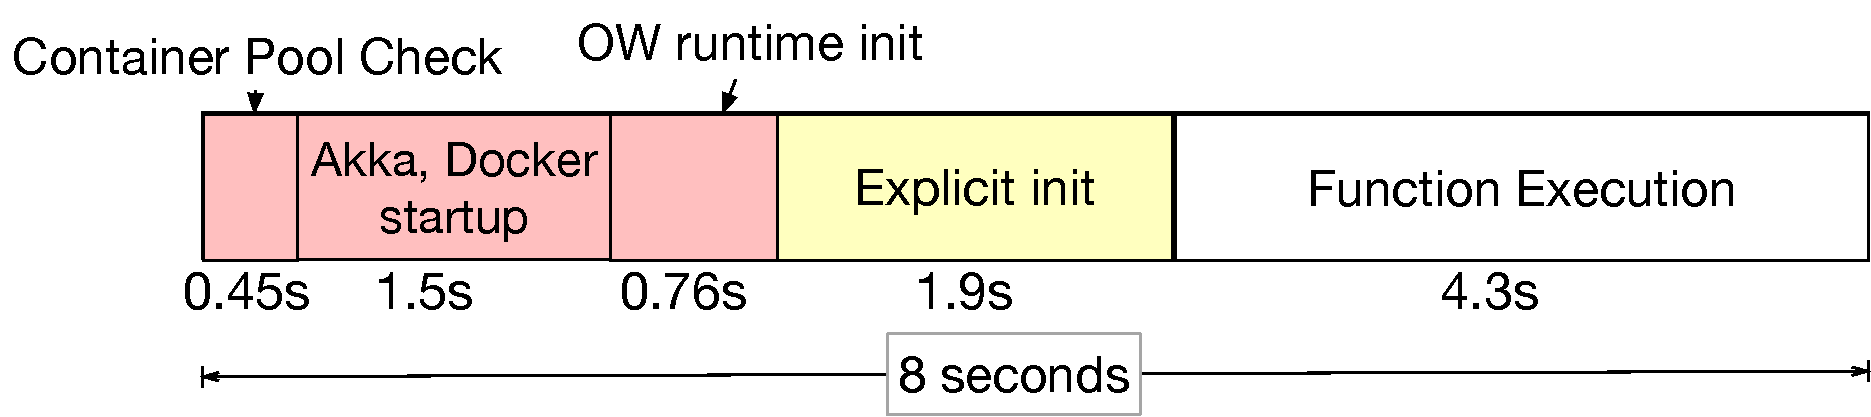
\includegraphics[width=0.8\textwidth]{faascache/faas-keepalive-20/figures/ow-timeline.pdf}
  \caption{Timeline of function execution and sources of cold start delay in OpenWhisk for an ML inference application.}
  \label{fig:timeline}
\end{figure}


\noindent \textbf{Function Initialization.}
%\noindent \textbf{Function Initialization.}
%
%Optionally, applications may also use custom code to initialize and pre-warm the container 
%rev1 first and last line 
%Explicit
Function initialization refers to function-specific code for downloading and resolving code and data dependencies, which can be run before actual function execution (explicit-init component in Figure~\ref{fig:timeline}). 
For example, this can be used for downloading data dependencies ahead of time such as large neural network models for inference, or for runtime initialization such as downloading and importing package dependencies (e.g., Python packages). 
%The second technique for reducing the cold start overhead is to explicitly initialize functions before running  them, and resolving most of the function's code and data dependencies during the initialization phase. 
%
An example of function initialization is shown in Figure~\ref{fig:lambda-example}, which shows a pseudo-code snippet of a function that performs machine learning inference on its input. 
For ML inference, the function downloads an ML model and initializes the TensorFlow ML framework (lines  5 and 6). 
If the function's container is kept alive, then invocations of the function do not need to run the expensive initialization code (lines 2--6). 
%Thus, the execution latency of functions can be minimized with a combination of careful function initialization and keeping the containers alive. 
% too broad a conclusion here...


% \footnotesize
\begin{figure}
\begin{lstlisting}[language=Python, numbers=left, frame=single, basicstyle=\footnotesize\sffamily, columns=fullflexible, xleftmargin=10.0ex, xrightmargin=10.0ex]
#Initialization code 
import numpy as np 
import tensorflow as tf
  
m = download_model('http://model_serve/img_classify.pb')
session = create_tensorflow_graph(m) 
  
def lambda_handler(event, context):
     #This is called on every function invocation 
     picture = event['data']
     prediction_output = run_inference_on_image(picture) 
     return prediction_output 
   \end{lstlisting}
   %\vspace*{\myfigspace}
   \caption{Initializing functions by importing and downloading code and data dependencies can reduce function latency by hiding the cold start overhead.}
   \label{fig:lambda-example}
   %\vspace*{\myfigspace}
\end{figure}


% The function cold start overhead includes both the execution environment initialization and the
\begin{comment}
Explicit initialization allows functions to be pre-warmed, and can be used to reduce the cold start overhead. 
However, explicit initialization is not common---our empirical investigation into FaaS benchmarks~\cite{kim_functionbench_2019} and official examples showed that applications do not use this functionality. 
Nevertheless, it can be a powerful technique to amortize expensive operations such as package imports and downloading data dependencies. 
Explicit initialization can thus increase the effectiveness of keep-alive. 
However because it is not ubiquitous, we assume it is \emph{optional}, and our keep-alive and provisioning techniques work with and without it. 
\end{comment}


\noindent \textbf{Workload Diversity and Dynamism.}
%
Designing keep-alive policies is not trivial due to the highly diverse and expanding range of applications that are using FaaS control planes.
%This is in tradeoffs category. 
Conventionally, FaaS has been used for hosting web services, which is attractive because of the pay-per-use properties. 
Event handling functions for web responses typically have a small memory footprint but require low execution latency. 
Increasingly, FaaS is also being used for ``heavy'' workloads with high memory footprint and large initialization overheads such as highly parallel numerical computing (such as matrix operations~\cite{jonas2017occupy}, scientific computing~\cite{shankar2018numpywren}, and machine learning~\cite{akkus_sand_2018}. 
The diversity of FaaS applications also results in a wide range of function memory footprints, running times, and initialization times, as seen in Table~\ref{tab:fc:workloads}.  
Keep-alive policies must therefore balance the resource footprint of the containers with the benefits of keeping containers alive---and do so in manner that is applicable across a wide range of applications. 


Furthermore, FaaS workloads show a high degree of dynamism and temporal effects. 
The Azure function~\cite{shahrad_serverless_2020} trace shows sharp diurnal effects: the function arrival rate is about $2\times$ higher during the peak periods compared to the average. 
Function workloads are also heavy-tailed: a few ``heavy hitting'' functions are invoked much more frequently than others or consume a larger amount of computing resources, often by 2 or 3 orders of magnitude. 


\subsection{Policy Goals and Considerations}


% The primary goal of keep-alive is to reduce the initialization and cold start latency, by keeping functions alive for different durations based on their characteristics. 
% % Servers that run these functions are heavily multiplexed, and run hundreds of short lived functions concurrently. %backend FaaS servers?
% % too sudden 
% Because servers run hundreds of short lived functions concurrently, keep-alive policies must be generalizable and yield high server utilization. 
% Functions can have vastly different characteristics, and keep-alive polices must work efficiently in highly dynamic and diverse settings. % (Table~\ref{tab:workloads}). 
% We use the following characteristics of functions for keep-alive policies.


% The \textbf{initialization time} of functions can vary based on the code and data dependencies of the function.  
% For example, a function for machine learning inference may be initialized by importing large ML libraries (such as TensorFlow, etc.), and fetching the ML model, which can be hundreds of megabytes in size and take several seconds to download. 
% Functions also differ in terms of their \textbf{total running time}, which includes the initialization time and the actual execution time. 
% Again, functions for deep-learning inference can take several seconds, whereas functions for HTTP servers and microservices are extremely short lived (few milliseconds). 
% The \textbf{resource footprint} comprises of the CPU, memory, and I/O use, and also differs widely based on the application's requirements. 
% Finally, functions have different \textbf{frequencies} and invocation rates. Some functions may be invoked several times a second, whereas other functions may only be invoked rarely (if they are used to serve a very low-traffic web-site, for instance). 

% \begin{figure}[t]
%   \centering
%   \vspace*{\myfigspace}
%   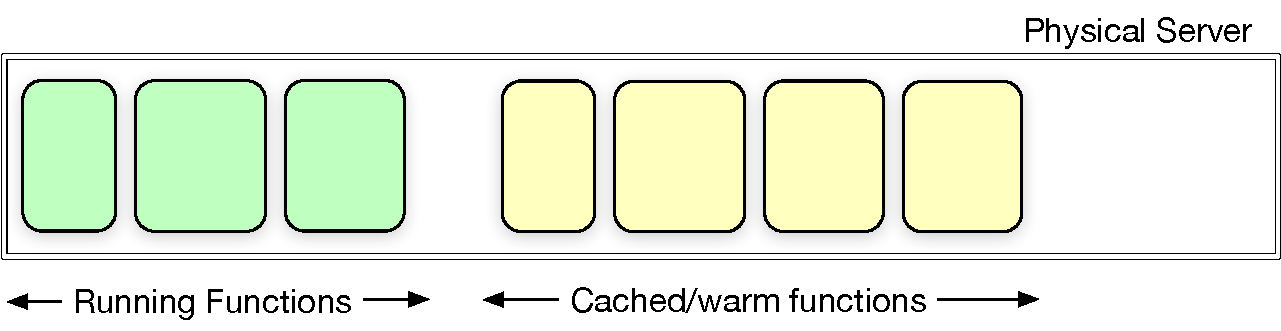
\includegraphics[width=0.4\textwidth]{../graphs/faas.pdf}
%   \vspace*{\myfigspace}
%   \label{fig:runwarm}
%   \caption{Server resources are consumed by running and warm containers.}
%     \vspace*{\myfigspace}
% \end{figure}


Because server resources are finite, it is important to prioritize functions which should be kept alive, based on their \textbf{initialization time}, \textbf{total running time}, \textbf{resource footprint}, and \textbf{frequencies}.
A function which is not popular and is unlikely to be called again in the near future, sees little benefits from keep-alive, and wastes server memory. 
%In fact, keeping such functions alive consumes valuable server computing resources for no gain in efficiency. %energy.. hmm
%Thus, keep-alive policies should prioritize popular functions. 
Similarly, the resource consumption of the functions is also important: since keeping large-footprint functions alive is more expensive than smaller functions, smaller functions should be preferred and kept alive for longer. 
Finally, functions can also be prioritized based on their initialization overhead, since it is effectively wasted computation.

% This paragraph is key. Different priorities and there is no one single ranking scheme for keepalive... 
The problem of designing keep-alive policies is complicated by the fact that functions may have vastly different keep-alive priorities across the different characteristics.
Consider a function with a large memory footprint (like those used in ML inference), high initialization overhead, and a low popularity.
Such a function should have a low keep-alive priority due to its size, high priority due to large initialization overhead, and a low priority due to its low popularity.
Thus, keep-alive policies must carefully balance all the different function characteristics and prioritize them in a coherent manner. 


% This still reads like making a case. But its only two sentences and bears repeating?
Current FaaS systems have shirked this challenge and use primitive keep-alive policies that are not designed with the diversity and dynamism in mind. 
FaaS frameworks such as OpenWhisk, keep all functions alive for a \emph{constant} period of time (10 minutes). 
This is agnostic to different function characteristics such as resource footprint and initialization overheads, and only loosely captures popularity. 
More principled approaches are needed, which we provide next. 



%%% Local Variables:
%%% mode: latex
%%% TeX-master: "paper"
%%% End:
